% use xelatex
\documentclass{beamer}

\usetheme{Warsaw}
\usecolortheme{beaver}

\usepackage{fontspec}
\usepackage[finnish,english]{babel}

\title[Smoke Gets in Your Eyes]{Pitch: Smoke Gets in Your Eyes}
\author{Sampo Savolainen \\Niclas Joswig \\Niko Ilomäki}
\institute{University of Helsinki}
\date{October 17, 2018}

\begin{document}

\begin{frame}[plain]
\titlepage
\end{frame}

\section{Motivation}

\begin{frame}{Wildfires}
\begin{itemize}
\item Wildfires have long been a problem in the U.S., especially on the West Coast.
\item It is a problem that is not likely to disappear
\item In fact, FiveThirtyEight wrote in July that ``Wildfires In The U.S. Are Getting Bigger''
\end{itemize}
\end{frame}

\begin{frame}{Air quality}
\begin{itemize}
\item At the same time, poor air quality is also a problem in the U.S.
\item Changes in air quality happen both due to the wildfires and because of other factors
\item The U.S. Environmental Protection Agency (EPA) collects large amounts of data on air quality all across the U.S.
\end{itemize}
\end{frame}

\section{Goals}

\begin{frame}{Goals}
\begin{itemize}
\item How well can we predict the maximal size of a wildfire from the data we have when it is first observed?
\item Can we trace changes in air quality back to local wildfires with high precision?
\item And together, can we accurately notify about coming changes in air quality based on wildfire observations?
\end{itemize}
\end{frame}

\section{Data}

\begin{frame}{Data}
\begin{itemize}
\item Kaggle provides a large database encompassing 24 years and 1.88 million wildfires in the U.S.
\item The wildfire data was originally collected by the U.S. Forest Service
\item The EPA publishes a variety of air quality data from 1980 to 2018.
\end{itemize}
\end{frame}

\begin{frame}[plain]
\begin{columns}[T]
\noindent
\begin{column}{0.5\textwidth}
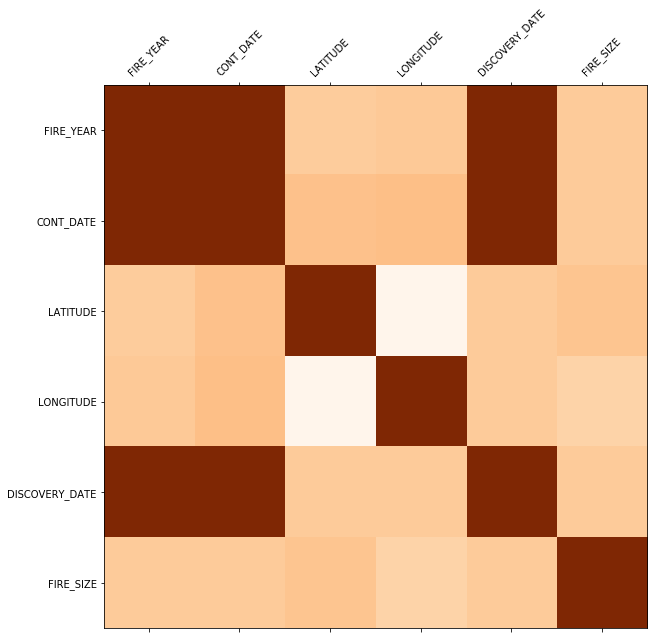
\includegraphics[width=0.95\textwidth]{correlation.png}
\end{column}
\hfill
\begin{column}{0.5\textwidth}
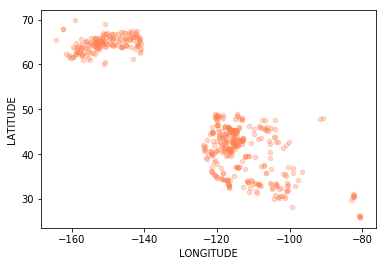
\includegraphics[width=0.95\textwidth]{map.png}

\noindent
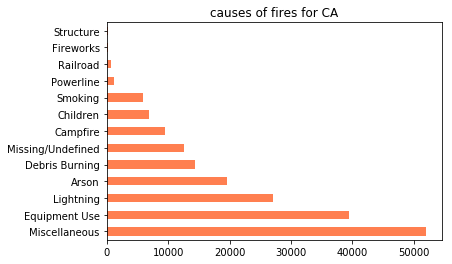
\includegraphics[width=0.95\textwidth]{fire_causes.png}
\end{column}
\end{columns}
\end{frame}

\section{Methods}

\begin{frame}{Methods}
\begin{itemize}
\item Multiple machine learning models will be evaluated for both parts of the project
\item In addition, combining the datasets requires building a model for how multiple wildfires would interact to change air quality at different distances from the fires
\end{itemize}
\end{frame}

\section{Bibliography}

\begin{frame}{Bibliography}
\begin{itemize}
\item Wildfire database: \\ \url{www.kaggle.com/rtatman/188-million-us-wildfires}
\item EPA air quality data: \\ \url{aqs.epa.gov/aqsweb/airdata/download_files.html}
\item FiveThirtyEight piece: \\ \url{fivethirtyeight.com/features/wildfires-in-the-u-s-are-getting-bigger/}
\end{itemize}
\end{frame}

\begin{frame}[plain]
\begin{center}
\LARGE Thank you!
\end{center}
\end{frame}

\end{document}
